\subsection{Megjelenítés}

%_
\begin{frame}
  A \texttt{display} tulajdonsággal állítható egy elem \emph{megjelenése}:
  \begin{description}[m]
    \item[\texttt{block}] \hfill \\ Blokkszintű megjelenítés
    \item[\texttt{inline}] \hfill \\ Soron belüli megjelenítés
    \item[\texttt{inline-block}] \hfill \\ Soron belüli blokk megjelenítés
    \item[\texttt{none}] \hfill \\ Nincs megjelenítés
  \end{description}
\end{frame}

%_
\begin{frame}
  \begin{description}[m]
    \item[Blokkszintű elemek] \hfill \\ Pl. \texttt{<p>}, \texttt{<div>}. Új sorban kezdődik, vízszintesen elfoglalja a teljes rendelkezésre álló helyet (átállítható).
    \item[Soron belüli elemek] \hfill \\ Pl. \texttt{<a>}, \texttt{<span>}. Sor (blokk) belsejében kezdődik, annyi helyet foglal, amennyit a tartalom kíván.
    \item[Soron belüli blokkok] \hfill \\ A két módszer vegyítése. Beállítható a szélesség, magasság, alsó és felső margók, kitöltések, mint a blokkszintű megjelenítésnél. Viszont az elem nem kerül új sorba. 
  \end{description}
  \vfill
  JavaScript programok gyakran használják a \texttt{none} értéket bizonyos tartalmak ideiglenes elrejtésére/megjelenítésére a DOM módosítása helyett.
\end{frame}

%_
\begin{frame}
  \begin{columns}[c]
    \column{0.66\textwidth}
      \begin{exampleblock}{\textattachfile{../css1/meretezes.html}{meretezes.html}}
        \scriptsize
        \lstinputlisting[style=HTML,linerange={7-17},numbers=left,firstnumber=7]{../css1/meretezes.html}
      \end{exampleblock}
    \column{0.3\textwidth}
      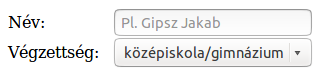
\includegraphics[width=\textwidth]{../css1/meretezes.png}
  \end{columns}
\end{frame}

%_
\begin{frame}
  \begin{columns}[c]
    \column{0.66\textwidth}
      A \texttt{visibility} tulajdonsággal állítható egy elem \emph{láthatósága}:
      \begin{description}[m]
        \item[\texttt{visible}] \hfill \\ Látható.
        \item[\texttt{hidden}] \hfill \\ Rejtett, de az elhelyezéséhez szükséges helyet a böngésző fenntartja!
      \end{description}
    \column{0.3\textwidth}
      \begin{exampleblock}{\textattachfile{display.html}{display.html}}
        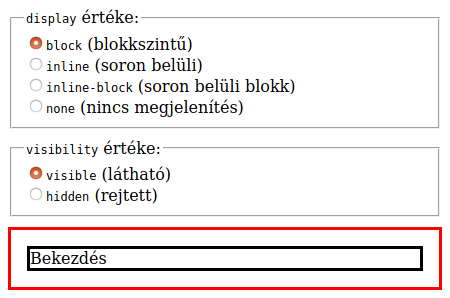
\includegraphics[width=\textwidth]{display.png}
      \end{exampleblock}
  \end{columns}
  
\end{frame}
